\begin{figure}[ht]
    \centering
    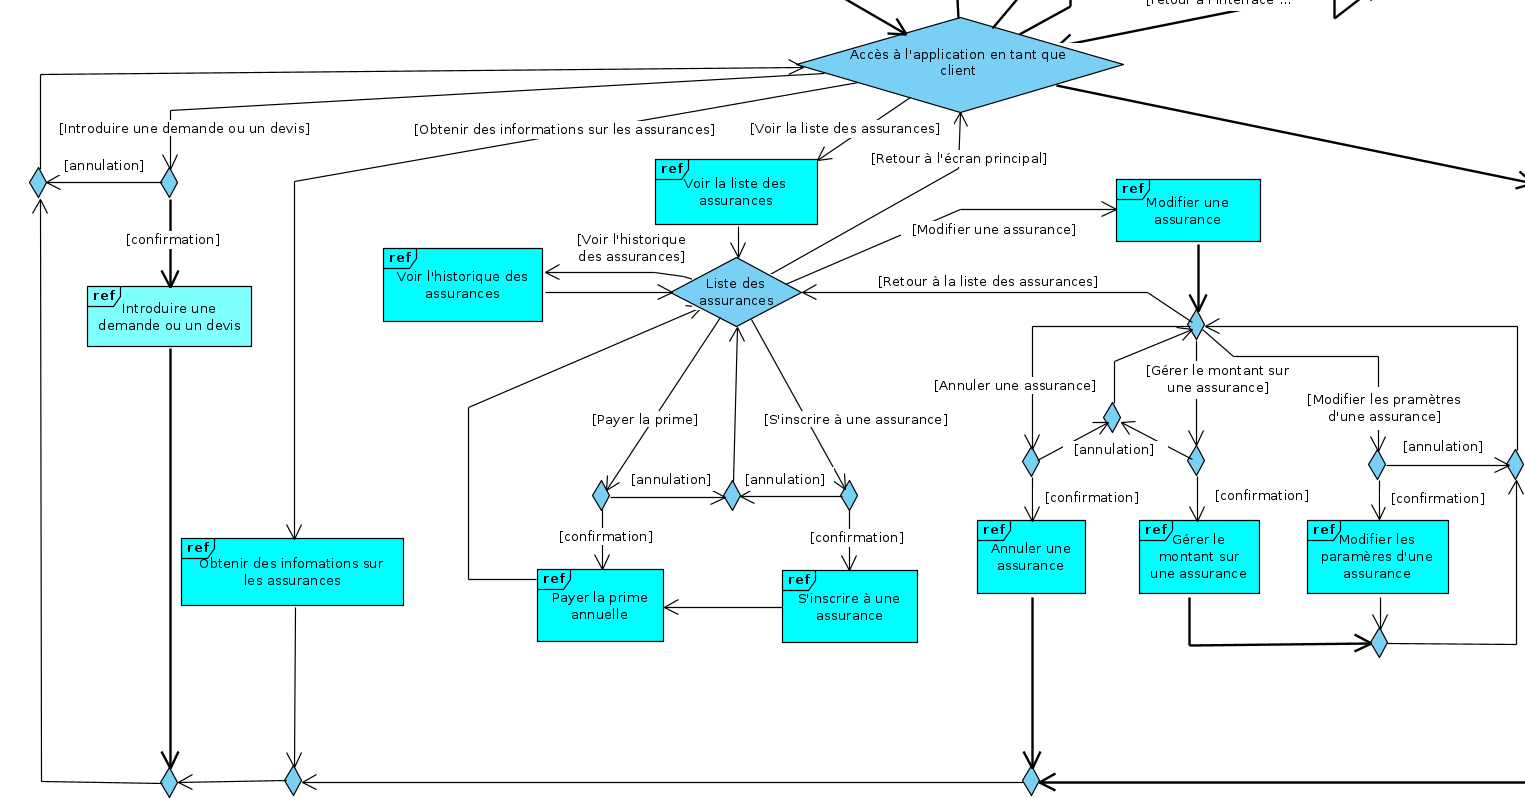
\includegraphics[scale=0.22]{img/InteractionDiagramClient.png}
    \caption{Ajout fait à l'Interaction Overview Diagram de l'application de base pour la partie client}
    \label{fig1}
    \end{figure}

\paragraph{}L’interaction overview diagram de l’extension assurance ajoute ses uses cases à celui de base. La grande partie de ceux ci sont disponibles après avoir listé les assurances. Après cela, on peut voir l’historique des assurances, s’inscrire à une assurance en payant la prime annuelle, payer la prime annuelle d’une assurance et modifier une assurance. Si l’on souhaite modifier une assurance, trois choix s’offrent à nous. Soit on peut annuler une assurance, soit gérer le montant sur une assurance, soit modifier les paramètres d’une assurance. A côté de cela on peut obtenir des informations sur les assurances et introduire un devis. Pour tout les cas importants, une confirmation est demandée avant d’effectuer l’action en question.
